\documentclass{beamer-control}
\usepackage{beamer-control-singlefile}
\INCLUDEONLY{PID Tuning}
\begin{document}
\CONCEPT{PID Tuning}

\begin{SUMMARY}
\begin{itemize}
\item Tuning laws
\item Automatic tuning
\end{itemize}
\vfill References:
\begin{itemize}
\item \astrom{§11.3}
\end{itemize}
\end{SUMMARY}



\SUBCONCEPT{Tuning laws}

\begin{frame}{Achieving desired response}
	\begin{itemize}
		\item Designers and users of control systems frequently need to adjust parameters to achieve some desired behaviour
		\item There are many, many ways to do this and one conventional framework is to model the system and then follow the design process outlined previously
		\item For complicated, high-dimensional, nonlinear systems this can often be a tedious process
		\item The PID controller has very few parameters and due to its simplicity may be preferrable in these challenging settings
		\item Empirical tuning laws based on real systems have been developed for the adjustment of control parameters
	\end{itemize}
\end{frame}

\begin{frame}{Ziegler-Nichols' tuning}
\begin{itemize}
\item Ziegler and Nichols designed the first tuning laws in the 1940s
\item The idea is to perform an experiment on the process dynamics, extract information about the system in the time and frequency domains, and infer good choices for the PID gains
\end{itemize}
\end{frame}


\begin{frame}{Ziegler-Nichols' tuning - Time-domain method}
\begin{itemize}
	\item In the time domain method, the step response of a system is measured by inputting a unit step and measuring the output (or scaling the output if the step was not of magnitude $1$)
	\item The output may be characterised by two parameters $a$ and $\tau$ and the resulting model is known as the Integrator with Time Delay (ITD) model
	\[P(s) = \frac{a}{\tau s}e^{-\tau s}\]
	\item The parameter $\tau$ approximates the time delay in the system and $\tfrac{a}{\tau}$ is the steepest slope of the step response
\end{itemize}
\end{frame}

\begin{frame}{Ziegler-Nichols' tuning - Time-domain method}
\begin{figure}
	\centering
	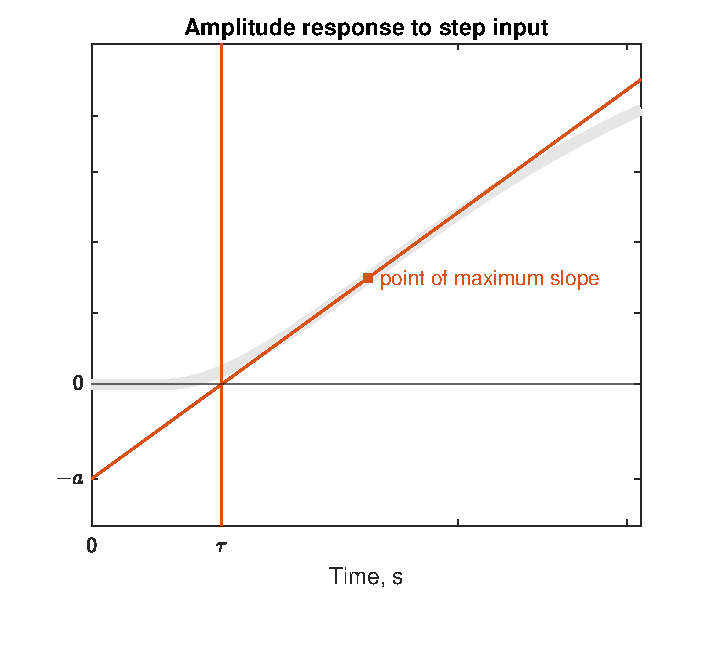
\includegraphics[width=8cm]{itd-at}
	\caption{Integrator with Time Delay (ITD) model.}
\end{figure}
\end{frame}

\begin{frame}{Ziegler-Nichols' tuning - Frequency domain method}
\begin{itemize}
	\item For the frequency domain version of Ziegler-Nichols' tuning laws a controller is connected to the system with integral and derivative gains set to $0$
	\item The proportional gain is increased until the system starts to oscillate
	\item At this point, the critical gain $k_c$ and the period of oscillation $T_c$ can be used to characterise the systems response
	\item From the Nyquist stability criterion, the loop transfer function $L(s)=k_cP(s)$ passes through the critical point at the frequency $\omega_c=\tfrac{2\pi}{T_c}$
	\item Therefore, we know the point on the Nyquist curve of the system $P(s)$ where the phase lag is $180^\circ$
\end{itemize}
\end{frame}


\begin{frame}{Ziegler-Nichols' tuning laws}
\begin{itemize}
	\item The suggested control parameters for both time and frequency domain methods are shown in Table 11.1
	\item These rules give a good starting point for manual tuning
	\item However, they are not very robust and don't use much of the information we get from the process transfer function
\end{itemize}
\begin{figure}
	\centering
	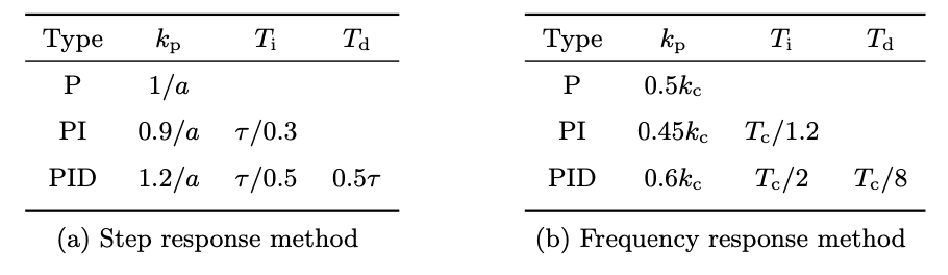
\includegraphics[width=\linewidth]{table11.1}
	\\
	\textbf{Table 11.1:} Ziegler-Nichols' tuning laws. 
\end{figure}
\end{frame}

\begin{frame}{FOTD tuning}
	\begin{itemize}
		\item We can improve the tuning of PID controllers by considering a characterisation of the system using a more descriptive model
		\item The first-order time-delay (FOTD) model
		\[P(s) = \frac{K}{1+sT}e^{-\tau s}\]
		can be used to approximate the step response of systems that achieve a steady state after a step input
		\item The relative time delay $\tau_n = \tfrac{\tau}{T+\tau}$
		has values between $0$ and $1$ and characterises the dynamics of the system
		\item If $\tau_n$ is close to $0$ the dynamics are lag dominated, if $\tau_n$ is close to $1$ the dynamcis are delay dominated, and the dynamics are said to be balanced for intermediate values of $\tau_n$
	\end{itemize}
\end{frame}




\begin{frame}{FOTD tuning - model}
\begin{figure}
	\centering
	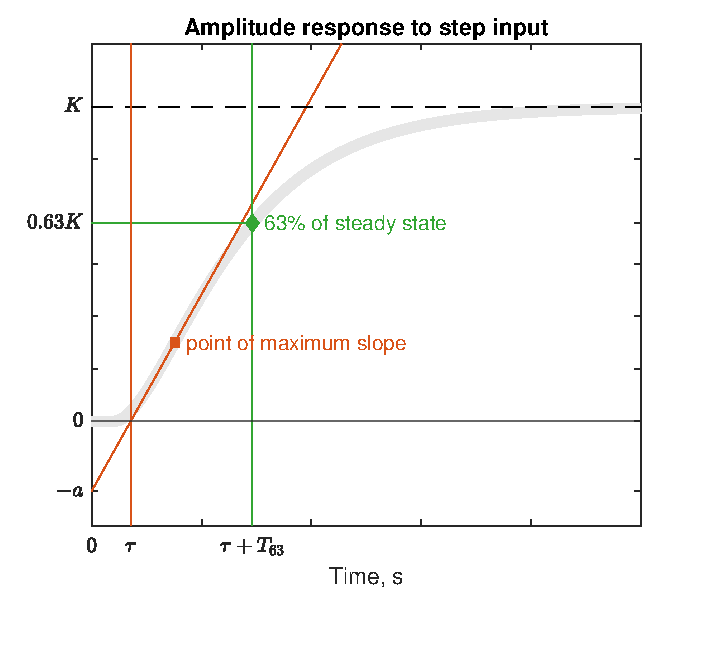
\includegraphics[width=8cm]{fotd-LT}
	\caption{First Order Time Delay (FOTD) model.}
\end{figure}
\end{frame}

\begin{frame}{FOTD tuning laws}
\begin{itemize}
	\item There are many tuning laws for FOTD models
	\item These typically give lower controller gains than the original Ziegler-Nichols' gains
\end{itemize}

\begin{columns}
\begin{column}{0.4\textwidth}
	\begin{table}
	\centering
	\begin{tabular}{|c|c|c|}
		\hline
		$K_p$ & $T_i$ & $T_d$\\
		\hline
		$\frac{0.6}{a}$ & $T$ & $\frac{\tau}{2}$\\
		\hline	
	\end{tabular}
	\caption{FOTD Chien-Hrones-Reswick tuning law (0\% overshoot)}
\end{table}
\end{column}

\begin{column}{0.6\textwidth}
			
\begin{table}
	\centering
	\begin{tabular}{|c|c|c|}
		\hline
		$K_p$ & $T_i$ & $T_d$\\
		\hline
		\tiny{$\frac{1.35}{a}\left(1 + \frac{0.18 \hat{T}}{1-\hat{T}} \right)$} & \tiny{$ \tau\left( \frac{2.5-2\hat{T}}{1-0.39\hat{T}} \right) $} & \tiny{$\tau \left( \frac{0.37-0.37\hat{T}}{1-0.81\hat{T}} \right)$}\\
		\hline	
	\end{tabular}
	\caption{Cohen-Coon tuning law where $\hat{T}=\frac{\tau}{\tau+T}$}
\end{table}
\end{column}
\end{columns}


\end{frame}


\SUBCONCEPT{Automatic tuning}

\begin{frame}{Relay feedback}
\begin{itemize}
\item In the Ziegler-Nichols' frequency domain method we increase the gain of the proportional controller until oscillation is achieved
\item We can obtain this information automatically by connecting a nonlinear element with a relay function in the feedback loop
\item For many systems, this will introduce oscillation where the relay output $u$ is a square wave, and the process output $y$ is close to a sinusoid
\item The input and outputs will be out of phase, meaning that the system oscillates with the critical period $T_c$
\item For relay amplitude $d$ and process output amplitude $a$, the critical gain is $k_c=\tfrac{4d}{\pi a}$ (by considering the first harmonic component of the Fourier series of $u$)
\end{itemize}
\end{frame}

\begin{frame}{Automating PID tuning with relay feedback}
\begin{itemize}
	\item This may be implemented into a system to achieve automatic tuning of the PID gains 
	\item The relay amplitude may be adjusted to keep oscillations sufficiently small
	\item Only a quick experiment for identifying the system is needed to find PID gains automatically and while the system is running
\end{itemize}
\begin{figure}
	\centering
	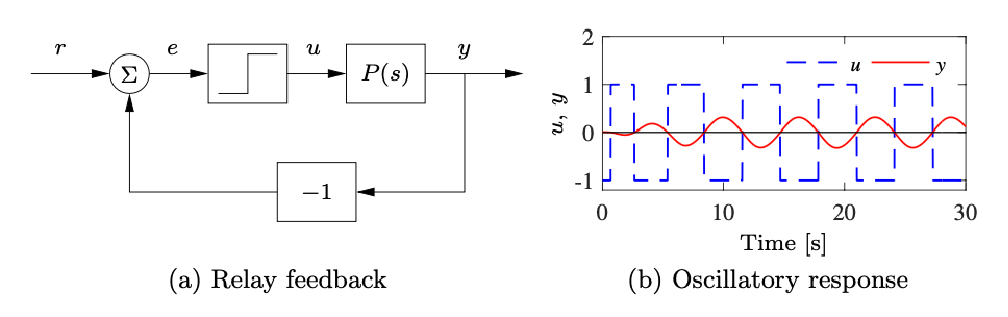
\includegraphics[width=0.8\linewidth]{figure11.9}
	\\
	\textbf{Figure 11.9}: Block diagram of a process with relay feedback (a) and typical signals (b).
\end{figure}
\end{frame}


\SUMMARYFRAME
\FINALE

\end{document}
